\section{Overview of Natural Language Processing}
Natural Language Processing (NLP) as a field covers a wide range of computational tasks that all relate to the concept of creating computer-based models of either some aspect of language or more ambitiously all aspects of language. These models are then normally used to create explicit structure for the vast quantities of text that contains only implicit structure. NLP tasks can be categorised based on the linguistic property that the tasks are addressing e.g. a syntactic or semantic task. These linguistic properties and  the related tasks are generally hierarchical, whereby knowing the output of a lower level task should help the higher level task. The low level syntactic tasks tend to be sequence labelling problems whereby each token\footnote{A token comes from tokenizing all words in the text using a tokenizer, of which this can cause some `words' to be broken up further to produce more than one token per `word'.} \citep{kaplan2005method,dridan-oepen-2012-tokenization} in the text (sequence) is assigned a label \citep{yannakoudakis-etal-2017-neural}, an example of this can be seen in figure \ref{fig:lit_review_constituency_tree} whereby each token is assigned a Part Of Speech (POS) tag. Examples of low level syntactic tasks are POS tagging \citep{church-1988-stochastic, ling-etal-2015-finding} and Chunking \citep{tjong-kim-sang-buchholz-2000-introduction}. The low level syntactic information is usually used to guide the higher level syntactic tasks such as dependency \citep{nivre-etal-2007-conll} and constituency parsing \citep{collins-2003-head}. As can be seen from the constituency and dependency trees within figure \ref{fig:lit_review_constituency_tree}\footnote{Constituency tree demo URL \url{https://demo.allennlp.org/constituency-parsing}} and \ref{fig:lit_review_dependency_parse_tree}\footnote{Dependency tree demo URL \url{https://demo.allennlp.org/dependency-parsing}} the POS tags correlate largely with the constituency and dependency labels e.g. a noun (\textit{NN}\footnote{Singular noun.}) being part of a noun phrase (\textit{NP}) and a noun (\textit{NNS}\footnote{Plural noun.} or \textit{NN}) being the modifier in the nominal subject modifier (\textit{NSUBJ}). The POS tags and constituency and dependency labels come from a limited tag or label set and the examples given here in figures \ref{fig:lit_review_constituency_tree} and \ref{fig:lit_review_dependency_parse_tree} come from the Penn Treebank POS tag set \citep{taylor2003penn}, syntactic tags of the Penn TreeBank \citep{taylor2003penn}, and Stanford typed dependencies \citep{de2008stanford} respectively.

The relation between lower and higher level syntactic tasks has been explicitly shown to be hierarchical within \citet{sogaard-goldberg-2016-deep} multi task learning\footnote{For an introduction into multi task learning and how it relates to transfer learning (which will be mentioned later in this section) see \citep{ruder2019neural} chapter 3 and 3.2.} work. The relation between tasks extends beyond the categories where syntactic information is useful for semantic based tasks, for instance within text classification. The example sentence within the figures is a neutral sentence as it contains an equal amount of positive and negative sentiment\footnote{If the sentence is put through Stanford CoreNLP 3.9.2 it would also classify the sentence as neutral. URL to Stanford CoreNLP 3.9.2 \url{https://corenlp.run/}}. To know the sentiment of the sentence it requires knowing that words such as \textit{great} are positive words, semantic knowledge. Further for the example sentence knowing that the words \textit{was n't} modifies the meaning of the word \textit{great} requires syntactic (from the dependency tree, figure \ref{fig:lit_review_dependency_parse_tree}) and semantic information. Similar to the syntactic tasks, semantic tasks also have a hierarchical structure where some tasks require less language understanding than others \citet{sanh2019hierarchical}. For a more comprehensive overview of syntactic and semantic tasks in NLP and how they relate, see Chapter 6 and 7 in \citet{goldberg2017neural}. In recent years it has been shown that utilising Neural Networks (NN) that have been initially trained on a high level NLP tasks such as Masked Language Modelling (MLM) \citep{devlin-etal-2019-bert} can be useful for the whole NLP pipeline (syntactic to semantic tasks) \citep{tenney-etal-2019-bert}. Thus finally showing how the tasks are hierarchical in nature. This brief primer into NLP does not touch on any topics that utilise NLP with any other modality, such as images for image captioning \citep{Karpathy_2015_CVPR}, audio for sentiment analysis \citep{raaijmakers-etal-2008-multimodal}, and many more, but these areas are out of scope for this thesis.

\begin{figure}[!h]
    \centering
    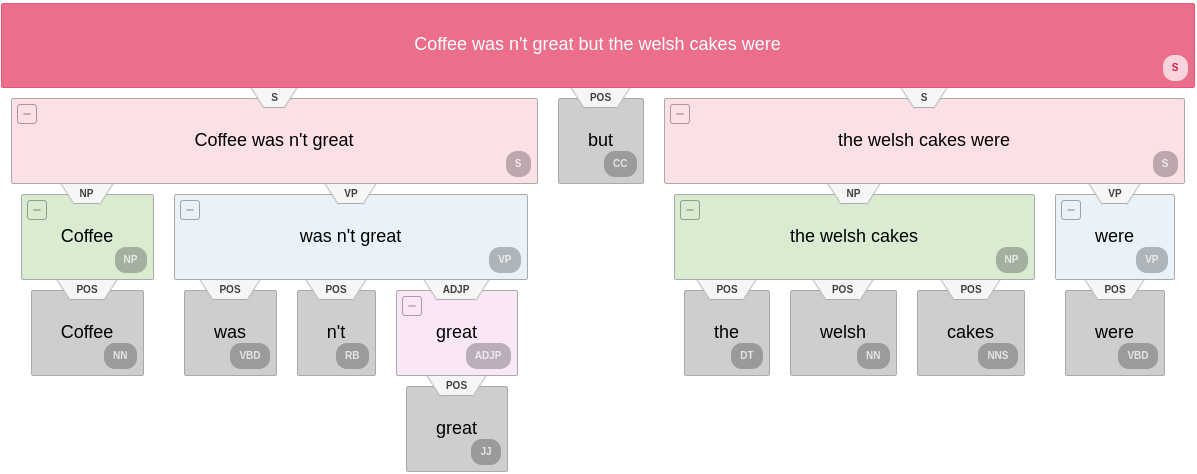
\includegraphics[scale=0.28]{images/lit_review/constituency_tree.png}
    \caption{Constituency tree for the sentence `Coffee wasn't great but the welsh cakes were'. The labels in each box represents the constituency label for that span, the labels for the leaf nodes are the POS tags for those words. The tree was created using the AllenNLP demo, which used \citet{joshi-etal-2018-extending} model.}
    \label{fig:lit_review_constituency_tree}
\end{figure}

\begin{figure}[!h]
    \centering
    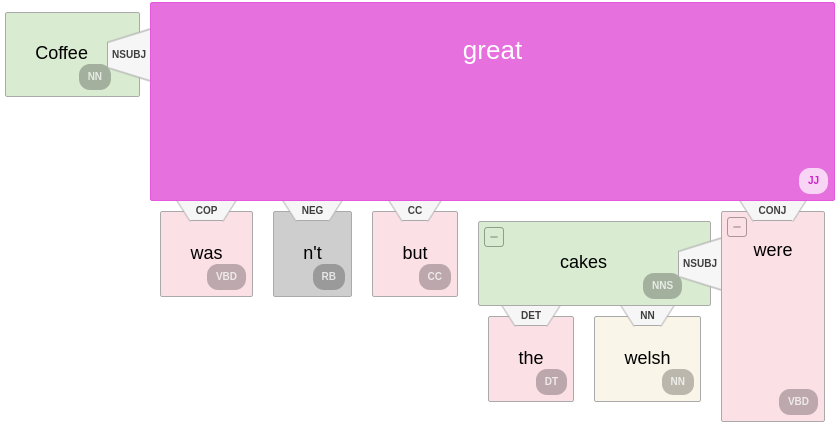
\includegraphics[scale=0.28]{images/lit_review/dependency_parse_tree.png}
    \caption{Dependency tree for the sentence `Coffee wasn't great but the welsh cakes were'. The labels within the arcs are dependency labels, and the labels within each box represents the POS tag for the given word. An arc from \textit{word A} to \textit{word B} indicates that \textit{B} is modifying \textit{A}, where \textit{A} is the head word. For example \textit{great} is the head word of \textit{coffee}. The tree was created using the AllenNLP demo, which used \citet{DBLP:conf/iclr/DozatM17} model.}
    \label{fig:lit_review_dependency_parse_tree}
\end{figure}

\section{Sentiment Analysis}
Sentiment analysis can be seen as a more general topic that contains multiple different sub-tasks. These tasks tend to be related and often have different assumptions. In this section, the different tasks within sentiment analysis  will be discussed. During the discussion some important concepts within NLP will also be introduced such as different neural network methods, domain adaptation and multi and cross lingual tasks. At the end of the section the different sentiment tasks will be explicitly shown in terms of how they are related to the main topic of this thesis which is Target Dependent Sentiment Analysis (TDSA).
% Need to mention at the end of this paragraph about poor evaluation and the lack of error analysis showing where alogrthims improve e.g. for generlaising to new targets or targets that exist but with different sentiment. something amybe about generlisation as well.

The many methods that have been used to tackle TDSA and all NLP problem fall into three different categories; supervised, unsupervised, and semi-supervised. Supervised methods require labelled data, in the case of sentiment analysis this would be sentiment label attached to their relevant text \citep{pang-etal-2002-thumbs}. Unsupervised methods on the other hand only require unlabelled data, which in the sentiment analysis case just the text. Unsupervised methods within sentiment analysis are normally based around sentiment lexicons (list of words that have an attached sentiment) \citep{hu2004mining} and sometimes a combinations of rules \citep{Hutto2014VADERAP}. Thus unsupervised methods tend to require some prior knowledge. Finally semi-supervised is a combination of the two learning from both the labelled data and extra unlabelled data \citep{zhu2005semi}. For a more complete overview of the differences between supervised, unsupervised and semi-supervised see \citet{Weston2007LargeScaleSL}.

\subsection{Document Sentiment Analysis}
The most common sentiment analysis task is that of document level. The task here is given a document which is made up of multiple sentences, to predict the sentiment. An example sample for this task can be seen in example \ref{example:lit_review_document_sentiment}. The first to apply a supervised machine learning algorithm to this problem was \citet{pang-etal-2002-thumbs}, where they applied several Machine Learning (ML) classifiers with Bag Of Words (BOW) as features to a new movie review dataset. This line of research of applying ML was further extended by \citet{pang-lee-2004-sentimental} who found that they could reduce the number of sentences by removing objective sentences in the document without significantly impacting, and in some cases improving, the overall accuracy of the classifier. \citet{mullen-collier-2004-sentiment} explored incorporating more semantic features into the BOW models such as the average sentiment values based on the unsupervised techniques of \citet{turney-2002-thumbs}. This approach of adding more semantic information into BOW models was further explored by \citet{whitelaw2005using} who created lexicon feature sets based around appraisal groups. Even though the use of semantic information had improved results \citep{whitelaw2005using}, the strong baseline performance of just using n-gram BOW features was further investigated by \citet{martineau2009delta} who showed that incorporating the class into the TF-IDF weighting mechanism \citep{jones1972statistical} to create Delta TF-IDF significantly improved results. However Delta TF-IDF was only created to work with two classes\footnote{In the sentiment case this is the positive and negative classes.} and not shown to generalise to \textit{n} classes. However a future study by \citet{paltoglou-thelwall-2010-study} showed that further performance gains can be made to TF-IDF based systems by using more enhanced weighting systems like BM25 \citep{robertson1995okapi}.

\begin{example}
\textit{a couple of criminals ( mario van peebles and loretta devine ) move into a rich family's house in hopes of conning them out of their jewels . however , someone else steals the jewels before they are able to get to them . writer mario van peebles delivers a clever script with several unexpected plot twists , but director mario van peebles undermines his own high points with haphazard camera work , editing and pacing . it felt as though the film should have been wrapping up at the hour mark , but alas there was still 35 more minutes to go . daniel baldwin ( i can't believe i'm about to type this ) gives the best performance in the film , outshining the other talented members of the cast .}
\caption{Negative document level sentiment example. Document ID \textit{cv435\_24355} taken from \citet{pang-etal-2002-thumbs} sentiment dataset.}
\label{example:lit_review_document_sentiment}
\end{example}

The supervised approaches that have been mentioned so far use a BOW approach, of which this form of vector representation is limited in what it can represent. BOW approaches that use n-gram word features can only learn what a word means within that \textit{n} window. For instance take \textit{n} to be 1 and 2\footnote{i.e. uni-gram and bi-gram features.} it would understand terms such as `very good' and `good' where both would be associated with positive sentiment, however if the statement was `not very good' then it would not capture the full sentiment as it would require all three words to know it is negated. One approach would be to have a very large value for \textit{n}, but this would create a very sparse vector representation which would not generalise well \citep{le2014distributed}. Thus the move away from BOW sparse vector representations to dense word representations was shown to be promising for sentiment analysis in \citet{maas-etal-2011-learning} work. However this work only found better performance than BOW when they combined the dense vectors with the BOW sparse vector. This first step into dense representation did show some promise as the representation can be learnt from unlabelled data, of which they found that results increased when more unlabelled data was used. These dense representations are very similar to what a traditional BOW model learns through its weights within the model \citep{goldberg2017neural}\footnote{See section 2.5.}. The benefit of using the dense representations on the downstream task (sentiment analysis) is that a good representation of the vectors can be learnt from another unsupervised task from unlabelled data first\footnote{The task can also be supervised, but would required labelled data.}. Thus allowing the model to have prior knowledge of what words mean (semantically and syntactically \citep{mikolov2013efficient}) encoded into the vector representation before training the model, unlike the BOW representation which contains no prior knowledge. 

\citet{le2014distributed} showed for the first time how dense vector representations using a NN could surpass BOW representation of which \citet{wang-manning-2012-baselines} set a high baseline at the time for a BOW method. \citet{le2014distributed} created dense document/paragraph vector representations that in comparison to the prior word level versions \citep{maas-etal-2011-learning} could encode document size texts without averaging by learning to predict the next word within a small context window from the document, thus each document vector would be different unlike the word representations\footnote{Unless two or more documents are identical.}. \citet{johnson-zhang-2015-effective} showed that without any additional unlabelled data unlike \citet{le2014distributed} a Convolution NN (CNN) can outperform the BOW approach. The CNN can be seen as a NN approach to a BOW model where by the CNN has a set of user defined window sizes of which these window sizes are analogous to n-grams in a BOW model. The CNN differs from the BOW model as it can generalise to unknown n-gram sequences, as it learns how to combine representation from multiple word representations to create the n-gram representation, rather than in the BOW case where it learns what that entire n-gram means and disregards similarities between n-grams based on the words within the n-gram. Furthermore the CNN model does not have the sparsity problem that a BOW model has thus the window size (n-gram in BOW case) can be large e.g. \citet{johnson-zhang-2015-effective} found that having a window size of 2 and 3 to perform best\footnote{\citet{le2014distributed} has a good summary of the drawbacks of BOW vector representations.}. For a more complete overview of CNNs, the reader is directed to chapter 13 of \citet{goldberg2017neural}.

None of the above methods, including the NN approach, take into account the word order of the whole document. One family of NN that explicitly encodes whole sequence of text in word order is the Recurrent NN (RNN) \citep{rumelhart1985learning}. The RNN has several popular variants; Long Short Term Memory (LSTM) \citep{hochreiter1997long} and the Gated Recurrent Unit (GRU) \citep{cho-etal-2014-learning}. \citet{dai2015semi} showed practically that LSTMs can be used for long sequence classification tasks such as document sentiment classification. \citet{xu-etal-2016-cached} created the Cached LSTM to better encode information from large sequences of text, like documents, and showed that it can outperform the LSTM on document sentiment analysis. Hierarchical \citep{zhang2015character} and dilated \citep{strubell-etal-2017-fast} CNN approaches have been created which can capture large contexts e.g. sentences rather n-grams, of which they have been shown successful in sentiment analysis \citep{conneau-etal-2017-deep}. Finally and more recently the transformer NN \citep{vaswani2017attention} approach has been applied which does not preserve word order (like the RNN or CNN) but rather treats the text more like a tree structure through attention mechanisms, whereby each word learns to contextualise itself within the text (can be the whole text). The transformer success can be best seen through BERT \citep{devlin-etal-2019-bert} where the architecture can be applied to task like document sentiment analysis \citep{sun2019fine}\footnote{For a good comparison of RNN, CNN, and transformer based models with respect to computational cost see section 4 of \citet{vaswani2017attention}.}. 

The majority of these more recent NN approaches have been tested on much larger sentiment datasets (100Ks documents) compared to the earlier work (2-25K documents). It has also been shown that for some of these NN approaches to work well they require extra data \citep{dai2015semi}. However it was found in \citet{dai2015semi} that these NN approaches can make great use of unlabelled data through a language modelling objective. This technique of training on one or more datasets and/or tasks before then applying the model to the end task (in this case document sentiment analysis) is defined as transfer learning in this thesis \citep{ruder2019neural}\footnote{Chapter 3}.  Both \citet{howard-ruder-2018-universal} and \citet{sun2019fine} found that by pretraining (a type of transfer learning) on the unlabelled data can have large performance gains, making the models more sample efficient with respect to labelled/annotated data. All of the neural methods within this and the last paragraph take into account large contexts of the document if not the whole document, whereas none of the previous methods could effectively do so. This allows the methods to overcome one the main challenges in document sentiment analysis that both \citet{turney-2002-thumbs} and \citet{pang-etal-2002-thumbs} found where the sentiment of the whole document is not the ``sum of the parts'' \citep{turney-2002-thumbs}.

The approaches taken so far treat the document as one large object to encode using some form of supervised method. However there have been methods proposed that suggest it is better to break the document up into smaller linguistic units to encode first into some form of intermediate representation, which is then later combined to generate a sentiment value for the whole document. \citet{bhatia-etal-2015-better} used Rhetorical Structure Theory (RST) \citep{mann-1984-discourse} to create a discourse structure for the document, of which this can be represented as a dependency-based discourse tree where the nodes are represented by Elementary Discourse Units (EDUs). They found that weighting the outputs of different supervised and unsupervised methods applied to EDUs in the tree based on their depth within the tree improved results. \citet{yang-etal-2016-hierarchical} used sentences to represent the whole document and weighted these sentences and the words within each sentence using two learnt attention mechanism. Thus this method unlike \citet{bhatia-etal-2015-better} learnt which sentences and words within those sentences where important to the document's sentiment rather than having a predefined weighting mechanism.

\citet{pang-etal-2002-thumbs} created the first English dataset of movie reviews (1.4K documents), which was later revised and increased in \citet{pang-lee-2004-sentimental} (2K documents), and then increased a lot further by \citet{maas-etal-2011-learning} (25K documents). The prior datasets all contained only two classes, positive and negative, of which these were based on the star rating that the movie review was given by the user. \citet{zhang2015character} created four much larger datasets ($~600$K - $~4$M documents) that have originated from Yelp\footnote{https://www.yelp.com/dataset} and Amazon reviews \citep{mcauley2015image} which contain between two and five classes where the classes are based around the user's star rating. This list of English datasets is not supposed to be exhaustive but is given as reference to popular and widely used datasets from the past and current literature.

In this sub-section, document sentiment analysis has been covered with respect to supervised methods and the associated popular English datasets. From the literature it is clear to see that the SOTA are NN based methods that require some form of transfer learning \citep{yang2019xlnet}. All of the methods also clearly point to one of the main challenges in document sentiment analysis which is the size of the documents. This can be seen from early in the literature where  \citet{turney-2002-thumbs} state that the sentiment of the whole document is not the `sum of the parts'. This therefore means that the whole document needs to be understood in context to fully understand the sentiment which has been shown not possible with the BOW methods. Thus the move to NN approaches such as the LSTMs, hierarchical CNNs, and transformers to overcome this problem. Finally within this sub-section different NN approaches have been explained as well as defining the concept of transfer learning.

\subsection{Sentence Sentiment Analysis}
Sentence level sentiment analysis is very similar to document whereby the only difference is the length of the text to be processed. Due to the length difference, the task is somewhat conceptually easier as a sentence is less likely to have multiple conflicting sentiments, thus the overall sentiment of the sentence is easier to predict. Many different approaches have been used for sentence based BOW \citep{wang-manning-2012-baselines}, CNN \citep{kim-2014-convolutional, kalchbrenner-etal-2014-convolutional}, LSTM \citep{brahma2018improved}, BERT \citep{devlin-etal-2019-bert}. However similar to document level, ``the sentiment of a sentence is not merely the sum of the polarity of the words and phrases found in the text, but rather depends on a number of compositional phenomena that act of indicators of polarity'' \citep{barnes2019improving}. This problem can be best seen in figure \ref{fig:lit_review_sentence_sentiment_example}\footnote{The sentence was chosen from \citet{barnes2019improving} and the figure was generated using the live demo found at this URL \url{http://nlp.stanford.edu:8080/sentiment/rntnDemo.html}.}, whereby it can be seen that even though the sentence has multiple positive words the sentiment of the sentence is dominated by the scope of the negation. Due to this, many approaches have been taken to better model the sentiment phrases within the sentence using BOW with compositional semantics \citep{choi-cardie-2008-learning}, Conditional Random Field (CRF) \citep{nakagawa-etal-2010-dependency}, Recursive NN (RCNN) \citep{socher-etal-2012-semantic} deep RCNN \citep{irsoy2014deep}, Tree-LSTM \citep{tai-etal-2015-improved}, Graph NN (GNN) \citep{zhang-zhang-2019-tree}, and multi task learning whereby negation scope and cue detection are the auxiliary task \citep{barnes2019improving}.

\begin{figure}[!h]
    \centering
    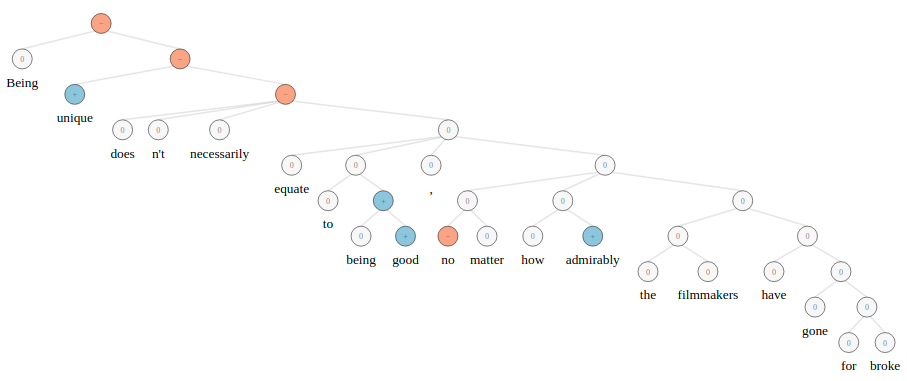
\includegraphics[scale=0.4]{images/lit_review/sentence_sentiment_example.png}
    \caption{Phrase and overall sentiment from \citet{socher-etal-2013-recursive} model, where by red, white, and blue represent negative, neutral, and positive sentiment respectively. The sentence in the figure is `Being unique doesn’t necessarily equate to being good, no matter how admirably the filmmakers have gone for broke'.}
    \label{fig:lit_review_sentence_sentiment_example}
\end{figure}

\citet{socher-etal-2013-recursive} took modelling phrases within sentences further by creating a dataset where by each phrase from the \citet{pang-lee-2005-seeing} movie dataset was manually annotated with a sentiment value, of which this can be seen in figure \ref{fig:lit_review_sentence_sentiment_example} whereby the model output shown is how the dataset is annotated. Thus this dataset allows models to better capture the compositional phenomena more explicitly by using the phrase level annotation. In a similar trend \citet{yang-cardie-2014-context} found that using inter and intra sentence discourse features to be useful showing that sentence level classification can be dependent on surrounding sentences. Taking that further \citet{mcdonald-etal-2007-structured} found that jointly modelling the sentence and document classification tasks helps improve both. More recently \citet{angelidis-lapata-2018-multiple} found that by framing document classification as a multiple instance learning (MIL) \citep{dietterich1997solving} problem they were able to create a sentence (EDU) classifier using only the document labels, this outperformed a fully supervised sentence (EDU) level classifier.  

This review has shown that sentence level sentiment requires both understanding the complex structure within the sentence as well as the more global content of the document. However even though the literature shows the use of explicitly taking into account phrases and document level information current SOTA uses the same techniques as that of document level \citep{yang2019xlnet}, utilising transfer learning mainly from a language modelling task. Even so \citet{barnes-etal-2019-sentiment} has annotated the errors coming from SOTA models into eighteen different categories finding that they perform badly on sentences containing non-standard spellings, idioms, and world knowledge to name a few. This shows that sentence level sentiment analysis still has plenty of error cases to solve through better incorporating linguistic and world knowledge into new and/or existing methods. To clarify all of the research mentioned on sentence level sentiment analysis was applied and thus to some extent developed for English. 

\subsection{Aspect Based Sentiment Analysis}
Document and sentence level sentiment analysis both assume that they are discussing one topic \citep{liu2015sentiment}\footnote{Page 47-48.}, for instance if the document (sentence) comes from a review (headline of a review) of the movie, \textit{The Avengers}, the topic that the sentiment is assumed to be about is the movie, \textit{The Avengers}. However both documents and sentences can contain sentiments on multiple different topics not just the main overall topic of the entire review. Aspect Based Sentiment Analysis (ABSA) attempts to overcome this problem by instead of predicting one sentiment for a document or a sentence it predicts multiple sentiments conditioned on multiple different predefined aspects/topics. ABSA can be performed at different linguistic granularities typically either document or sentence level. Example \ref{example:lit_review_document_aspect_sentiment} a Tripadvisor review taken from \citet{Wang2010LatentAR} with seven aspects and their respective sentiments\footnote{They were actually ratings rather than sentiments, but the ratings are used as approximations for sentiment.}, as well as the overall sentiment of the hotel. From this document level ABSA example it can be seen that these aspects are latent, that is the aspect itself does not necessarily occur in the text, this is shown in example \ref{example:lit_review_document_aspect_sentiment} where by the \textit{service} is negative as the ``Hotel staff speak zero English... The process at the hotel is a bit confusing... staff weren't overly friendly.''. This example would be typically used as a training example for document level ABSA.  


%Further this example demonstrates that even though the overall sentiment can be negative other aspects can be positive, like the \textit{value} of the hotel. Thus illustrating why document and sentence level sentiment analysis is too coarse and why a more fine grained approach like ABSA is required. 

\begin{example}
\textit{Good and clean but no English spoken The good: The hotel is in a great location and withing walking distance to the Forbidden City and some other sights in this hisrotic district. The rooms were comfortable and clean, really good value.The bad: Hotel staff speak zero English. Breakfast is only Chinese breakfast. The process at the hotel is a bit confusing (make sure you keep those pink receipts they give when you pay, you need them to check out!) and staff weren't overly friendly. Internet is expensive and slow.}
\caption{Example of document level aspect sentiment analysis. The aspects and their receptive sentiments are: \textit{service} (1), \textit{business service} (2), \textit{cleanliness} (3), \textit{check in / front desk} (2), \textit{value} (4), \textit{rooms} (3), and \textit{location} (4). The sentiments were on a scale of 1-5 and the overall sentiment for the review was 2. This was taken from review id \textit{447367} from the trip advisor review dataset of \citet{Wang2010LatentAR}.}
\label{example:lit_review_document_aspect_sentiment}
\end{example}

\citet{snyder-barzilay-2007-multiple} treated the task of document ABSA as a supervised ranking problem, where each aspect is ranked based on a BOW feature vector. They showed the benefit of modelling dependencies between aspects. They found that 38\% of their restaurant review training data contained the same sentiment for all aspects in the there respective reviews. Thus they added an agreement function within their model which predicts whether or not all aspects for the review should contain the same sentiment which significantly improved performance. In comparison \citet{Wang2010LatentAR} created the Latent Rating Regression model, which instead of learning from the aspect sentiments can train the model just from the overall sentiment. This therefore reduces the requirement of more fine grained sentiment training data, but the model did require a set of seed words that represented the aspects e.g. for the aspect \textit{room} a set of key words would be \textit{room}, \textit{suite}, \textit{view}, and \textit{bed}. 

More recently supervised Neural Network (NN) approaches have been the most popular and successful approach to document ABSA. The first to use a NN for document ABSA was \citet{lei-etal-2016-rationalizing}, of which their main aim was to create rationals/explanations for the predictions given only the aspect sentiment labels for supervision. \citet{yin-etal-2017-document} showed the importance of biasing the attention mechanism within a hierarchical NN \citep{yang-etal-2016-hierarchical} towards the aspect of interest. The attention mechanism used a set of keywords to define each aspect, from these keywords the attention mechanism would use a memory network \citep{weston2014memory} to learn how to best describe the aspect so that the model focused on the most important words and sentences in the document. \citet{yin-etal-2017-document} benchmarked their approached across numerous neural and non-neural approaches. \citet{li-etal-2018-document} used a similar hierarchical NN as \citet{yin-etal-2017-document} and found significant performance gains when incorporating both user\footnote{On the dataset that contained user information.} and/or the overall document sentiment information into the attention network. They found that the document sentiment information is useful as the related aspect sentiments are correlated. Further the user information allows the model to better capture textual and sentiment similarities at the aspect level e.g. a user tends to have similar sentiment scores for aspects across documents and tends to describe aspects in a similar manner across documents. Finally the most recent and successful approach used a hierarchical neural Reinforcement Learning (RL) \citep{williams1992simple} method \citep{wang-etal-2019-human}\footnote{They called document ABSA, Document-level Aspect Sentiment Classification (DASC).}, where by instead of splitting the document into sentences they used Elementary Discourse Units (EDUs). They used the RL approach to first find aspect relevant EDUs and then within the EDU the relevant aspect sentiment words. They found that if they had used sentences instead of EDUs\footnote{They call EDUs clauses.} then the performance would have decreased by 2.44\% on average, of which they believe this is due to 90\% of EDUs only containing one sentiment\citep{bayoudhi2015sentiment}. Through error analysis they found that their method performed poorly when negation is used or a comparison is made, however they did not quantify the number of times these errors where made.
% I think we should talk here about sentence level ABSA as the AE literature evaluates some what on both.

% There is also the SemEval review level datasets
There are three main datasets to evaluate document ABSA, TripAdvisor \citep{Wang2010LatentAR}\footnote{This is sometimes called TripDMS.}, BeerAdvocate \citep{mcauley2012learning}, and TripUser \citep{li-etal-2018-document}. Both the TripAdvisor and BeerAdvocate datasets since have been reprocessed by \citet{yin-etal-2017-document} so that aspect sentiments per document are less correlated\footnote{The standard train, development, and test splits for the TripAdvisor and BeerAdvocate datasets can be found here \url{https://github.com/HKUST-KnowComp/DMSC}.}. This technique of reducing the correlation of the aspect sentiments per document was suggested by \citet{lei-etal-2016-rationalizing}, to ensure that the model does not get ``confused''. It has not been shown whether training models on datasets that have less correlation between aspect sentiments per document produce better models, further \citet{snyder-barzilay-2007-multiple} actually exploited this correlation in their modelling. The TripAdvisor and TripUser are both hotel reviews from the Tripadvisor website\footnote{\url{https://www.tripadvisor.co.uk/}} and contain the same seven aspects, but the TripUser dataset also contains user information unlike TripAdvisor. The BeerAdvocate dataset comes from a beer review website Beeradvocate\footnote{\url{https://www.beeradvocate.com/}} and contains four aspects.

% Need to talk about some point the use of document level as a summary of sentence level which is useful for review websites.
The datasets mentioned so far are all the datasets that have been used\footnote{Or derivatives of.} in the prior work stated in this thesis so far. However these datasets are not expertly annotated data, rather the data has been scraped from there representative websites where the reviews were `annotated' by many different users. One of the few datasets that has been annotated by experts is the SemEval 2016 task 5 subtask 2 dataset \citep{pontiki-etal-2016-semeval}, of which it contains seven datasets in six different languages and vary across three domains\footnote{Restaurant, laptop, and hotel reviews.}. The only methods that have been applied to these datasets are those that entered the SemEval competition.\\

Sentence ABSA unlike document tends to contain far fewer aspects within it's text and unlike document it's rare for a sentence to have all aspects, which is not the case in document ABSA \citep{snyder-barzilay-2007-multiple, Wang2010LatentAR}. All document ABSA methods could be applied to sentence ABSA with minimal changes, however the vast majority of them have been designed for longer texts, for instance the hierarchical NN methods \citep{yin-etal-2017-document, li-etal-2018-document, wang-etal-2019-human}. To further iterate this point on a sentence containing few aspects per sentence examples \ref{example:lit_review_sentence_aspect_sentiment_1} and \ref{example:lit_review_sentence_aspect_sentiment_2} show two different sentences from the widely used SemEval 2014 task 4 subtask 4 restaurant review dataset \citep{pontiki-etal-2014-semeval}, each containing one and two aspects respectively. Further the statistics from the SemEval 2014 restaurant training dataset state that on average each sentence will only have 1.22 aspects\footnote{This was calculated based on the training datasets containing 3041 sentences of which in total there are 3713 aspects within that dataset.} \citep{pontiki-etal-2014-semeval}. In comparison to document, sentence ABSA is less likely to have an \textit{overall} sentiment\footnote{\textit{Overall} sentiment here refers to sentence or document level sentiment, rather than an \textit{overall/general} aspect sentiment e.g. the aspect \textit{RESTAURANT\#GENERAL} in the SemEval 2015 task 12 restaurant dataset\citep{pontiki-etal-2015-semeval}.}, of which some document approaches have made use of this \citep{Wang2010LatentAR, li-etal-2018-document}. Lastly document ABSA in affect summarises the sentiment information for each aspect that has been captured throughout the document, which can make document sentiment analysis a more difficult task if there are lots of contradicting sentiment for one aspect \citep{pontiki-etal-2016-semeval}.  


\begin{example}
\textit{Even though its good seafood, the prices are too high.}
\caption{Example of sentence level aspect sentiment analysis. Contains two aspects \textit{food} and \textit{price} with positive and negative sentiment respectively. This was taken from sentence id \textit{3440} from the trail restaurant dataset of \citet{pontiki-etal-2014-semeval}.}
\label{example:lit_review_sentence_aspect_sentiment_1}
\end{example}

\begin{example}
\textit{Overall I would recommend it and go back again.}
\caption{Example of sentence level aspect sentiment analysis. Contains one aspect \textit{anecdotes/miscellaneous} with positive sentiment. This was taken from sentence id \textit{2609} from the trail restaurant dataset of \citet{pontiki-etal-2014-semeval}.}
\label{example:lit_review_sentence_aspect_sentiment_2}
\end{example}

Sentence ABSA was popularised by task 4 in SemEval 2014 \citep{pontiki-etal-2014-semeval} where 20 teams created various methods. The winner \citet{kiritchenko-etal-2014-nrc} used a Support Vector Machine (SVM) \citep{chang2011libsvm} with different BOW features including ngrams, POS tags, and various in and out of domain sentiment lexicon features\footnote{Sentiment lexicon is a collection of different groups of words where each group is associated to a specific sentiment.}. Further to better capture the aspect specific sentiment they utilised a domain adaptation technique \citep{daume-iii-2007-frustratingly} such that each aspect category had it's own BOW weight vector that was learnt at the same time as the general BOW weight vector, so that aspect specific and general features can be learnt separately. SemEval repeated a similar task for two more years 2015, and 2016, of which the winners all use a similar BOW approach \citep{saias-2015-sentiue, brun-etal-2016-xrce, kumar-etal-2016-iit}. 

NN approaches for this task are desirable due to them requiring fewer linguistic resources, and the ease of transferring the approach to multiple languages \citep{ruder-etal-2016-insight-1}. \citet{ruder-etal-2016-insight-1} applied a CNN to the task outperforming many of the aforementioned BOW approaches on multiple languages. In later work \citet{ruder-etal-2016-hierarchical} showed that taking into account the surrounding sentences using an hierarchical LSTM further improved results. \citet{wang-etal-2016-attention} found that by adding attention to a sentence level LSTM improved the model by allowing it to better capture relevant aspect specific words within the sentence. Follow on work \citep{bao-etal-2019-attention} found that regularising the attention network using sentiment lexicons and/or attention sparsity improved the robustness of the model. \citet{wang2018aspect} utilised a hierarchical NN similar to \citet{yin-etal-2017-document} (document ABSA) where by the hierarchy of the sentence was based around EDUs within the sentence, and the words within those EDUs. This was proposed on the premise that EDUs often discuss one aspect, thus making the task for the NN easier, as the model could ignore EDUs that were not discussing the relevant aspect. They found this hierarchical approach to outperform the flattened version.

Popular sentence ABSA datasets for English are the SemEval 2014\footnote{The restaurant ABSA dataset partially came from \citet{Ganu2009BeyondTS}.}\citep{pontiki-etal-2014-semeval}, 2015\citep{pontiki-etal-2015-semeval}, and 2016 datasets for the laptop, restaurant, hotel review domain\footnote{The 2014 datasets ABSA annotation was only provided for the restaurant domain.}. A large difference between the 2015 dataset compared to the 2014 was the sentiment of an aspect may require a larger context than just the sentence the aspect appeared in, hence why the whole review was given as context.   


For a good overview of cross-lingual approaches to sentiment analysis at both the sentence and target level see \citet{barnes2019cross} thesis.

\citet{marcheggiani2014hierarchical} used a CRF model with various BOW features for aspect identification and sentiment prediction, where by they found jointly modelling the aspect and overall review sentiment to be beneficial for aspect sentiment prediction but not identification. Further they also introduced a sentence level English ABSA dataset with review/document level annotation for the hotel domain. 
%Adding user information into sentiment analysis methods has been done

In a similar line of work Aspect Extraction (AE) is the task of predicting the aspects that the text is discussing, again AE can also be performed typically at document or sentence level. In example \ref{example:lit_review_document_aspect_sentiment} the review has a set of predefined aspects, but not all reviews will always have all of these predefined aspect some may have fewer aspects, and in other domain like Laptop reviews may contain more aspects. For document AE \citet{titov2008modeling} created Multi-grain LDA (MG-LDA) a modified version of Latent Dirichlet Allocation (LDA) for the task of unsupervised document AE. MG-LDA compared to LDA creates two groups local and global where by they found that a local groups better correspond to aspects. To empirically validate their method they showed that adding the MG-LDA features to the \citet{snyder-barzilay-2007-multiple} model improved results and also out performed using the LDA features instead. The drawback of topic modelling methods like LDA or MG-LDA is the requirement of setting the number of topics that the model is required to generate, and then having to manually label which topics correspond to which aspects, if the topics do correspond to any of the predefined aspects. In comparison to this completely unsupervised approach \citet{mukherjee-liu-2012-aspect} used a set of seed words and known number of aspects/topics to constrain their topic modelling based method, which is similar to \citet{Wang2010LatentAR}. 

% A problem with all of these topic modelling based approaches is that it cannot assign a document/text to an aspect or a number of aspects without, the most interesting part of these type of clustering is that it can define what words are in what aspect clusters.
% The existing models that do use seeds can also generate more topics that have not been seeded and they judge if the topic is relevant by looking at the terms in the topic and judging using human knowledge.
More recent approaches have moved away from topic modelling like LDA to Neural Networks (NN). \citet{he-etal-2017-unsupervised} used an autoencoder styled unsupervised learning objective where by the NN was trained to reconstruct the encoded sentence from a dense matrix that would represent aspects. From this aspect matrix they could find words associated to an aspect using a similarity function between the aspect matrix and a word's vector representation/embedding. Further they could also assign a text to a single aspect label\footnote{The method could not assign more than one label to a text. This could be done but would require some form of threshold/confidence level on the output of the softmax in equation 6.} based on the output of the NN. This approach was later improved upon by \citet{angelidis-lapata-2018-summarizing} where the aspect matrix was initialised using a weighting approach from the embeddings of known aspect seed words, these seed words and their weighting did come from a limited amount of labelled data. Further they showed the benefit of using a multi task learning objective where by predicting the domain of the sentence\footnote{In this work instead of sentences they used EDUs.} was beneficial, as they believed domain relevant words were also relevant to the aspect. 

\citet{karamanolakis-etal-2019-leveraging} showed how to better utilise known aspect seed words through a student-teacher distillation model \citep{bucilua2006model, hinton2015distilling}, where by the teacher predicted the probability of each aspect for a sentence based on the frequency of the aspect seed words in the sentence\footnote{A special version of a BOW model.}. The student model then learnt off the teacher's model predictions thus not requiring any human annotated data. The teacher's model was then updated using the student predictions on the training data in a co-training setup \citep{blum1998combining}. Thus allowing the teacher to learn weights for each of the seed words, this improved teacher model then re-taught the student model, of which this process is then repeated until the predictions from the teacher and student are similar. The student model is then used to predict which aspect occurs in the text. The advantage of this student model approach unlike the previous NN approaches \citep{he-etal-2017-unsupervised, angelidis-lapata-2018-summarizing} it allows the student model to be any type of model. However they found that averaging word vectors similar to \citet{he-etal-2017-unsupervised, angelidis-lapata-2018-summarizing} to perform well and outperforms all existing unsupervised approaches\footnote{Approaches that use seed words tend to be called weakly supervised rather than unsupervised. This is due to the approach requiring some knowledge that has had to come from a human annotator. However in this part of the literature review we have grouped the unsupervised and weakly supervised together and have explicitly stated at each point if the method required seed words.}.
% next prehaps talk about different ways these are evaluated, may need to introduce the sentence level stuff.

In all of the previous work ABSA and AE has been discussed at the document level. However there are some noticeable problems with performing at this granularity. For AE, if the set of predefined aspects is known, like the seven aspects in example \ref{example:lit_review_document_aspect_sentiment}, then in most cases due to the size of the documents most of the aspects will be within the document thus making the task 

To overcome the problem that aspects can have multiple sentiments throughout a document or a sentence \citet{lazaridou-etal-2013-bayesian} setup the AE and ABSA task at the Elementary Discourse Unit (EDU). They also performed their analysis at this linguistic unit as they hypothesised that either the aspect and/or sentiment that the unit will be discussing will change at the start of an EDU. They found that incorporating knowledge of this aspect/sentiment change into their weakly supervised LDA model for AE and ABSA improved results. However performing AE and/or ABSA at EDU level never progressed any further than this line of work.

%A sample of sentence and Tweet can be seen in example. The reason for grouping both sentence and Twitter based methods is due to the fact that Tweet based methods can be seen as a adaptation of sentence based method to a different type of text. 


%The main difficulty in document sentiment analysis has been shown through it's length Further sentiment lexicons have been defined and numerous NN methods have been introduced. 

%So far the supervised methods within document sentiment analysis have been covered, from which it is clear to see that the SOTA are NN based and require some form of transfer learning \citep{yang2019xlnet}. All of the methods also clearly point to one of the main challenges in document sentiment analysis is the size of the documents. This can be seen from early in the literature where  \citet{turney-2002-thumbs} state that the sentiment of the whole document is not the `sum of the parts'. This therefore means that the whole document needs to be understood in context to fully understand the sentiment which has been shown not possible with the BOW methods. Thus the move to NN approaches such as the LSTMs, heirahcical CNNs, and transformers to overcome this problem.


%can be used to c encode some form of word order within 
%The use of dense vector representations stayed at the forefront to State Of The Art (SOTA) document sentiment classification. 

% created a much large movie review sentiment dataset \citet{maas-etal-2011-learning}
%who explored different information retrieval weighting mechanisms

%\citet{whitelaw2005using} Created a apprisal lexicon through using a list of words that were known to be part of the lexicon as `seed words' and then expanding that list through collocations, WordNet, and thesauri

%Incorporating 

%The first document sentiment dataset was by \citet{pang-etal-2002-thumbs}, which was then later enlarged by \citet{pang-lee-2004-sentimental}

%This novel Machine Learning (ML) work was conducted at the same time as \citet{turney-2002-thumbs} who applied an un-supervised approach to the same problem, both came across the same problem, which is that the sentiment of the review cannot be determined through `sum of it's parts' \citep{turney-2002-thumbs}\footnote{This is paraphrased for grammatical reasons, the actual quote is `sum of the parts'}. This problem is due to both works only using BOW (up to bi-grams) features within their methods, thus their features only take into account local context and limited linguistic knowledge (POS tags in \citet{turney-2002-thumbs}). This problem to some extent started to be alievated with the raise of more 

\section{Target Dependent Sentiment Analysis}
The holder within TDSA can be first related back to \citet{wiebe-1990-identifying} where they first explain in multiple different circumstances who the holder of the sentiment\footnote{In the original work they never used `sentiment' but rather `subjectivity' although the two are rather similar in these circumstances.} is and the difference between the holder and the target\footnote{In the original work they used the word `experiencer' rather than `target'}. In this work they also stated the importance of co-reference resolution\footnote{co-reference and anaphora resolution within this thesis are the same task.} with respect to finding the holder and how it can span over multiple sentences.

The first to state the importance of using Target Dependent (TD) over non-TD methods\footnote{Non-TD method is any method where given a text will return only one sentiment for that text, no matter if the text contains different sentiments for the targets within that text. An example of these non-TD methods would be document/sentence/tweet sentiment analysis.} for TDSA was \citet{jiang-etal-2011-target} where they find 40\% of samples\footnote{Out of a total of 100 samples.} to be mis-classified by the non-TD method due to it finding the overall sentiment of the sample rather than the sentiment for the target within the text.  

\section{Sentiment Summarisation}
In this section sentiment summarisation is reviewed as it relates significantly to the area of sentiment analysis and thus creates a better overview of the area of sentiment analysis. However this thesis does not contribute in any way to sentiment summarisation. Document level sentiment analysis summarisation attempts to re-write the review such that the main sentiments from the review are expressed in a more condensed review. \citet{angelidis-lapata-2018-multiple} created a system based on MIL so that EDUs (sentences) within the review have their own sentiment rating using only document sentiment labels. Using an attention mechanism they ranked the EDUs (sentences) and displayed the top percentage of these EDUs (sentences) as summaries of the document. They found in comparison to a similar system that does not use MIL \citep{yang-etal-2016-hierarchical} that there system is more informative and contains the better sentiment summary based on human evaluation. This is most likely due to the MIL method allowing EDUs (sentences) to be labelled as a opposite sentiment to that of the document label. Further they found that using EDUs to be better than sentences as summaries, which has also been shown in other summarisation work \citep{li-etal-2016-role}. 